\documentclass[11pt]{article}
\usepackage{fancyhdr}
\usepackage{graphicx}
\usepackage{amssymb}
\usepackage{epstopdf}
\usepackage{amsmath} 	
\usepackage{amssymb}
\usepackage{cite}
\usepackage{multirow}
\usepackage{wrapfig}
\usepackage{subfigure}
\usepackage{todonotes}
\usepackage{listings}
\usepackage{dtklogos}
\usepackage[colorlinks=true, linkcolor=black,citecolor=black,urlcolor=blue]{hyperref}
\bibliographystyle{IEEEtran}
\DeclareGraphicsRule{.tif}{png}{.png}{`convert #1 `dirname #1`/`basename #1 .tif`.png}


%---------------- Letter Paper --------------------%
% be sure to change in document class too
\textwidth = 6.5 in
\textheight = 8.5 in
\oddsidemargin = 0.0 in
\evensidemargin = 0.0 in
\topmargin = 0.0 in
\headheight = 0.0 in
\headsep = 0.2in
\parskip = 0.2in
\parindent = 0.0in


\begin{document}
\thispagestyle{empty}
\begin{center}
\vspace*{1.5in}
{\LARGE \textbf{Mini-Project 1}} %<---- Insert your project title here

{\Large MCHE 485: Mechanical Vibrations\\ \vspace*{0.1in} Spring 2016}

\vspace*{2.5in}

% author names and CLIDS
\begin{figure}[!h]
\begin{minipage}{0.45\textwidth}
\begin{center}
Matthew Begneaud \\
Department of Mechanical Engineering\\
University of Louisiana at Lafayette\\
Lafayette, LA 70504\\
{\tt mjb4932@louisiana.edu}
\end{center}
\end{minipage}
\hspace{0.08\textwidth}
\begin{minipage}{0.45\textwidth}
\begin{center}
Jace Delcambre\\
Department of Mechanical Engineering\\
University of Louisiana at Lafayette\\
Lafayette, LA 70504\\
\tt{jad5032@louisiana.edu}
\end{center}
\end{minipage}
\end{figure}

% Force some spacing for the third author
\vspace{0.2in}
\begin{figure}[!h]
\begin{minipage}{0.45\textwidth}
\begin{center}
Hayden Lejeune \\
Department of Mechanical Engineering\\
University of Louisiana at Lafayette\\
Lafayette, LA 70504\\
{\tt hjl2491@louisiana.edu}
\end{center}
\end{minipage}
\hspace{0.08\textwidth}
\begin{minipage}{0.45\textwidth}
\begin{center}
Travis \\
Department of Mechanical Engineering\\
University of Louisiana at Lafayette\\
Lafayette, LA 70504\\
\tt{CLID4@louisiana.edu}
\end{center}
\end{minipage}
\end{figure}
\end{center}

\newpage
\thispagestyle{empty}
\begin{abstract}
\vspace{-0.2in}
In the analysis of mechanical systems, vibrations are bound to occur. Many systems are quite complex, so finding the system characteristics, such as the natural frequency and damping ratio, are not trivial. However, these characteristics can be analyzed and estimated given data from recording the vibration of the system. In this report, the natural frequency and damping ratios of four systems are estimated using various system identification methods after trimming the recorded data to include only the clean portion of free vibration of the system.
\end{abstract} 

\newpage

% reset the page counter, so it begins with the page of the introduction section
\setcounter{page}{1} 


%%%%%%%%%%%%%%%%%%%%%%%%%%%%%%%%%%%%%%%%%%%%%%%%%%%%%%%%%%%%%%%%
%%%%%%%%%%%%%%%%%%%%%%%%%%%%%%%%%%%%%%%%%%%%%%%%%%%%%%%%%%%%%%%%
\section{Introduction}
\label{sec:intro}
\vspace{-0.2in}
The data retrieved from a particular system can be hard to interpret because of excessive noise clouding the results. Because of this it is important to clean up the data as much as possible before attempting to get accurate values from it. In this report, the data will be trimmed to only include the portion where free vibration is observed and will then be smoothed to decrease the effect of noise on the calculations. The processed data will be used to calculate the natural frequency of the system using zero-crossing analysis and FFT, as well as the damping ratio by peak analysis.
\bigskip

Data recorded from four systems is provided for this project. The raw data is then run through a python program that takes the data as input and performs the necessary calculations and plots the results. The plots include raw data, smoothed data, zero crossings and peak analysis, and FFT. An example plot showing zero crossings and peaks can be seen in Figure 1.
\bigskip
	
\begin{figure}[htbp] %  figure placement: here, top, bottom, or page
   \centering
   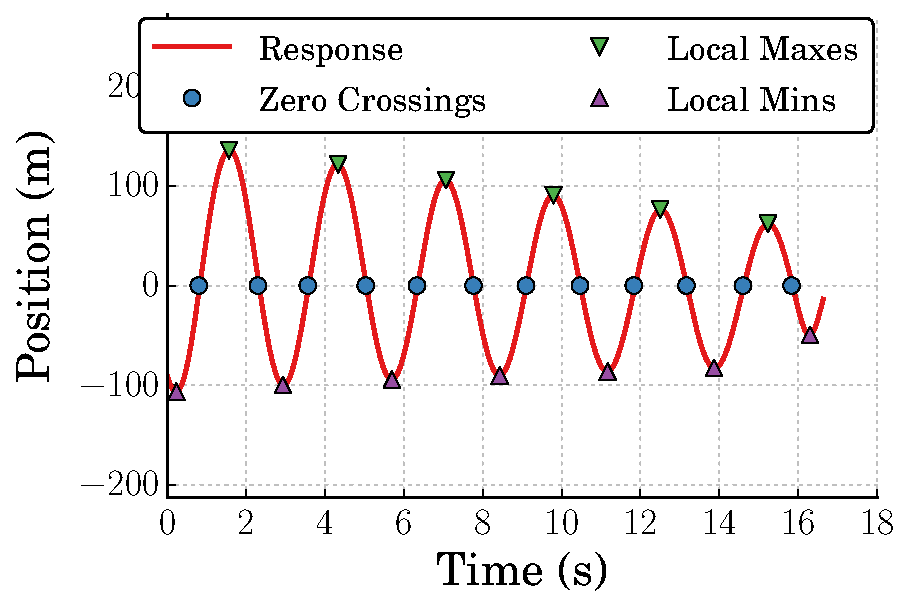
\includegraphics[width=4.5in]{zeroCrossings_and_extrema.pdf} 
   \caption{Zero Crossings and Local Extrema}
   \label{fig:example}
\end{figure}

\bigskip

The natural frequency can be estimated by zero-crossings analysis using the period of oscillation, defined as the time between zero crossings of similar slopes by using Equation 1. The natural frequency can be calculated using either one period, or multiple periods and taking the average value. Using multiple periods gives a more accurate result as it encompasses more data. 
\bigskip


\begin{equation}
\omega_{n} = \frac{2\pi}{\tau}
\label{eqn:example}
\end{equation}

\bigskip

The natural frequency can also be estimated using the Fast Fourier Transform (FFT), a fast and computationally inexpensive program used to perform Fourier analysis on a signal. An example of an FFT plot is shown in Figure 2.
\bigskip

\begin{figure}[htbp] %  figure placement: here, top, bottom, or page
   \centering
   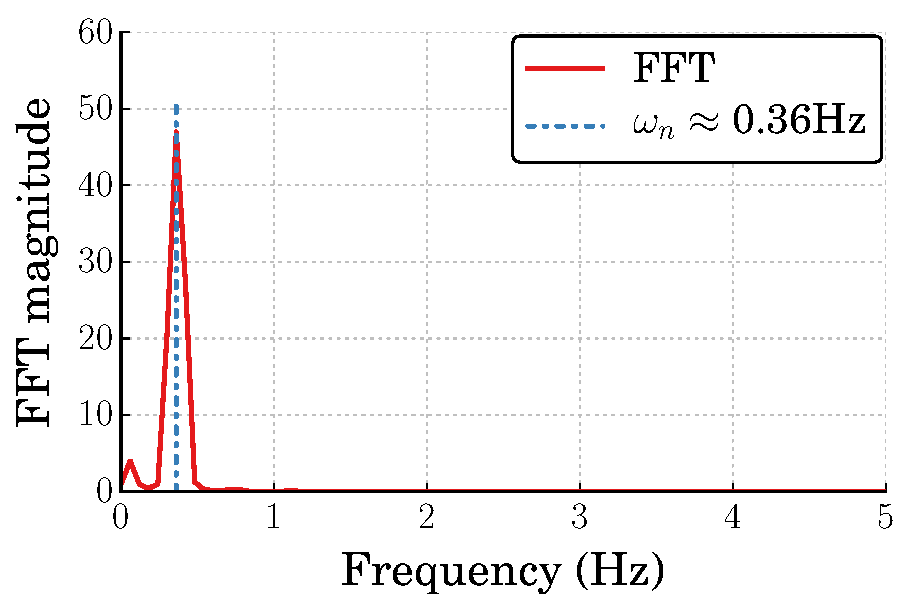
\includegraphics[width=4.5in]{FFT_magnitude.pdf} 
   \caption{FFT Analysis Plot}
   \label{fig:example}
\end{figure}

\bigskip

The damping ratio of the system can be estimated by analyzing the local minima and maxima (peaks) of oscillation during free vibration. In order to do so, $\sigma$ must be calculated by using Equation 2, where $x(0)$ is the value of the first peak (positive or negative) and $N\tau$ is the peak observed $N$ periods after the initial peak. After $\sigma$ is calculated, it can be used in Equation 3 to calculate $\zeta$. 

\begin{equation}
\sigma = \frac{1}{N}ln\left(\frac{x(0)}{x(N\tau)}\right)
\label{eqn:example2}
\end{equation}

\bigskip

\begin{equation}
\zeta = \frac{\sigma}{\sqrt{4\pi+\sigma^2}}
\label{eqn:example2}
\end{equation}



%%%%%%%%%%%%%%%%%%%%%%%%%%%%%%%%%%%%%%%%%%%%%%%%%%%%%%%%%%%%%%%%
\section{Results}
\label{sec:section_2_label}
\vspace{-0.2in}
%

The processed data (trimmed and smoothed) from data sets 1 through 4 can be seen in Figure 3 through Figure 6. The data was trimmed to exclude any initial inputs/impulses provided to the system, as well as any portions of data at the end of free vibration which became noisy and/or irregular. The results calculated by the program using processed data for each data set are shown in Table 1. 

\newpage

% Figures will go here
\begin{figure}[h!] %  figure placement: here, top, bottom, or page
   \centering
   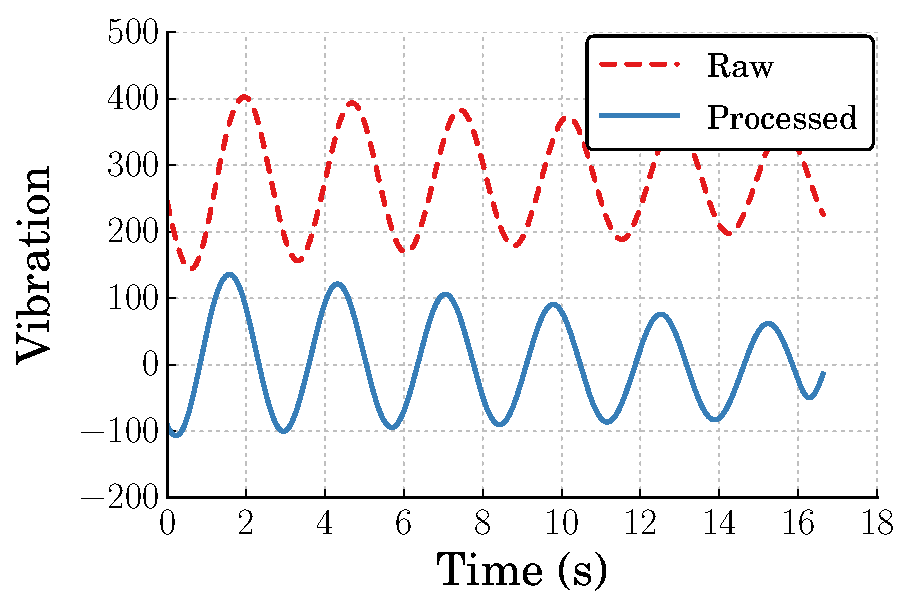
\includegraphics[width=5in]{vibration_data1.pdf} 
   \caption{Data 1}
   \label{fig:example}
\end{figure}

\bigskip

\begin{figure}[h!] %  figure placement: here, top, bottom, or page
   \centering
   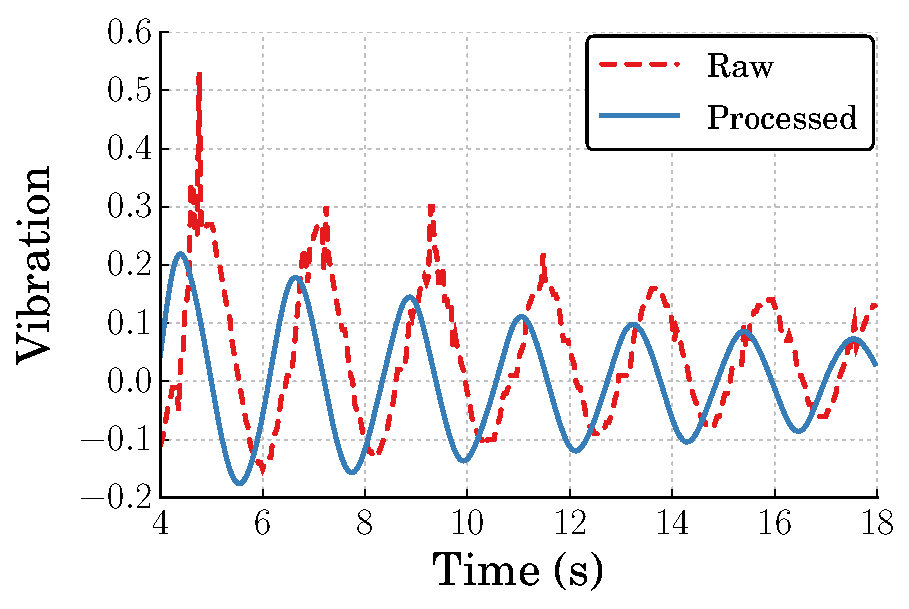
\includegraphics[width=5in]{vibration_data2.pdf} 
   \caption{Data 2}
   \label{fig:example}
\end{figure}

\newpage

\begin{figure}[h!] %  figure placement: here, top, bottom, or page
   \centering
   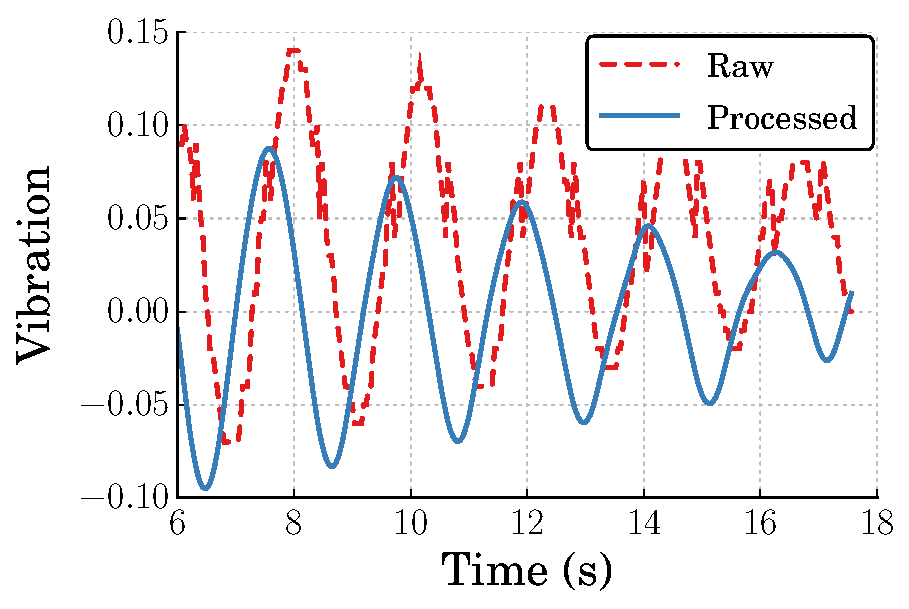
\includegraphics[width=5in]{vibration_data3.pdf} 
   \caption{Data 3}
   \label{fig:example}
\end{figure}

\bigskip

\begin{figure}[h!] %  figure placement: here, top, bottom, or page
   \centering
   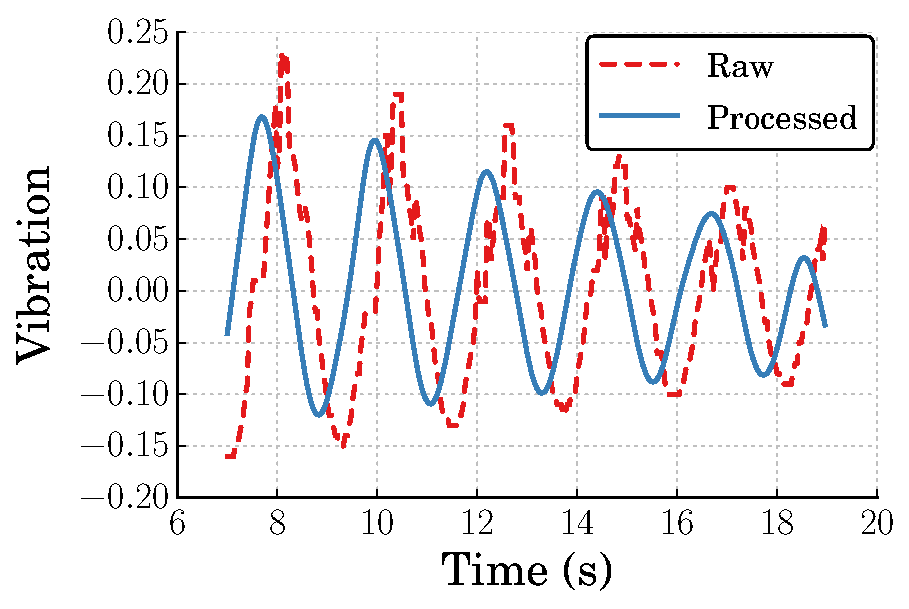
\includegraphics[width=5in]{vibration_data4.pdf} 
   \caption{Data 4}
   \label{fig:example}
\end{figure}

\newpage


\begin{table}[h!]
\centering
\caption{Results}
\bigskip
\label{my-label}
\begin{tabular}{cccccc}
\hline
\multicolumn{1}{l}{\textbf{Data Set}} & \textbf{\begin{tabular}[c]{@{}c@{}}$\omega_{n}$ (Hz)\\  (Zero Crossings)\end{tabular}} & \textbf{\begin{tabular}[c]{@{}c@{}}$\omega_{n}$ (Hz)\\ (FFT)\end{tabular}} & \textbf{\begin{tabular}[c]{@{}c@{}}$\zeta$\\ (pos. peaks)\end{tabular}} & \textbf{\begin{tabular}[c]{@{}c@{}}$\zeta$\\ (neg. peaks)\end{tabular}} & \textbf{\begin{tabular}[c]{@{}c@{}}$\zeta$\\ (log dec.)\end{tabular}} \\ \hline
1                                     & 0.3652                                                                                 & 0.3614                                                                     & 0.0249                                                                        & 0.0202                                                                        & 0.0226                                                                      \\
2                                     & 0.4575                                                                                 & 0.4310                                                                     & 0.0291                                                                        & 0.0229                                                                        & 0.0260                                                                      \\
3                                     & 0.4630                                                                                 & 0.4340                                                                     & 0.0402                                                                        & 0.0410                                                                        & 0.0406                                                                      \\
4                                     & 0.4482                                                                                 & 0.4195                                                                     & 0.0529                                                                        & 0.0154                                                                        & 0.0341                                                                     
\end{tabular}
\end{table}
\bigskip

It can be seen that the damping ratio for the third data set should be higher than that of the first two data sets, as the vibration decays more quickly. The results seen in Table 1 agree with this estimation, which reflects the results should be moderately accurate. The natural frequency calculated by use of zero-crossings analysis also seems to closely match the results calculated by the FFT program. It should be noted that the natural frequencies calculated by the program are more accurately defined as the damping frequencies, because the systems recorded in each data set are damped.
\bigskip

The damping ratios for data sets one, two, and three were consistent when using maxima and minima, however the values calculated for data set four varied more greatly between maxima and minima analysis. The average therefore may not be as accurate as the averages found in data sets one, two, and three.
\bigskip


%%%%%%%%%%%%%%%%%%%%%%%%%%%%%%%%%%%%%%%%%%%%%%%%%%%%%%%%%%%%%%%%
\section{Conclusion}
\label{sec:conclusion}
\vspace{-0.2in}
In this report, four sets of data are trimmed and smoothed. This processed data was then used to calculate the natural frequency and damping ratio of each system. The natural frequency was calculated using zero-crossings analysis as well as FFT analysis. The damping ratios were also calculated by using local extrema. The natural frequencies calculated by both methods closely match for all systems. The damping ratios for data sets one, two, and three were consistent by using maxima and minima, however data set four was found to be inconsistent between maxima and minima analysis.






\end{document}